\documentclass[a4paper,12pt]{article}
\usepackage[utf8]{inputenc}
\usepackage{graphicx}
\usepackage{subcaption}
\usepackage{amsmath}
\usepackage{amsfonts}
\usepackage{amssymb}
\usepackage{hyperref}
\usepackage{float}
\usepackage{geometry}
\usepackage{tabto}
\geometry{margin=1in}
\usepackage{csquotes}
\usepackage{listings}
\usepackage{xcolor} 
\usepackage{tcolorbox}


\lstset{
    language=Matlab, % The language of the code
    basicstyle=\ttfamily\small, % The basic font style used
    keywordstyle=\color{blue}\bfseries, % Style for keywords
    commentstyle=\color{green}, % Style for comments
    stringstyle=\color{red}, % Style for strings
    numbers=left, % Where to put line numbers
    numberstyle=\small\color{gray}, % Style for line numbers
    stepnumber=1, % Line number step size
    numbersep=10pt, % Space between line numbers and code
    backgroundcolor=\color{lightgray!10}, % Background color for the code block
    frame=single, % Frame around the code block
    breaklines=true, % Automatic line breaking
    captionpos=b % Caption position (b for bottom, t for top)
}

\tcbset{
  observation/.style={
    colback=yellow!10!white, % Background color
    colframe=black, % Border color
    fonttitle=\bfseries, % Title font
    coltitle=black, % Title color
    boxrule=0.5mm, % Border thickness
    title=Observation, % Title text
    sharp corners, % Sharp corners
    enhanced, % Allows more features
    attach boxed title to top left={yshift=-2mm, xshift=2mm},
    boxed title style={colframe=black, colback=yellow!30!white, boxrule=0.5mm},
  }
}


\tcbset{
  mybox/.style={
    colback=blue!5!white, % Background color
    colframe=blue!75!black, % Border color
    fonttitle=\bfseries, % Title font style
    boxrule=0.5mm, % Border thickness
    sharp corners, % Sharp corners
    enhanced, % Enhanced features
  }
}


\tcbset{
  historicalbox/.style={
    colback=yellow!10!white, % Background color
    colframe=orange!85!black, % Border color
    fonttitle=\bfseries, % Title font style
    title=Historical Curiosity, % Title of the box
    boxrule=1mm, % Border thickness
    sharp corners, % Sharp corners for the box
    enhanced, % Allows for more features
    coltitle=black, % Title color
    left=2mm, right=2mm, top=2mm, bottom=2mm, % Padding
    width=\textwidth, % Box width
    arc=2mm, % Corner rounding
  }
}

\begin{document}

\title{Control of Cyber-physical Systems\\ \vspace{0.5cm} \large LABORATORY WORK REPORT | PART II\\ \vspace{0.5cm} \large Computer Control of a Flexible Robot Arm Joint\begin{center}
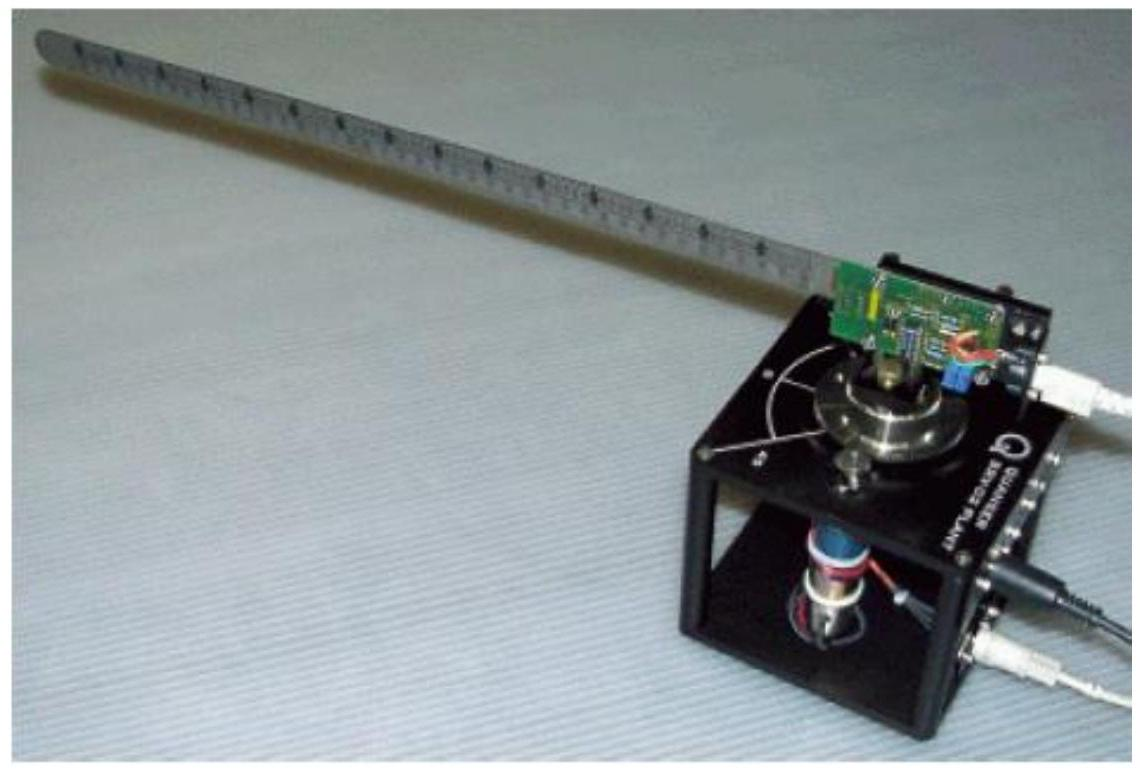
\includegraphics[width=0.6\textwidth]{Figs/2024_08_29_9e657742dc855ba919cag-01}

\vspace{15pt}
\emph{Shift L03} %% insert here the number of the shift you have attended
\end{center}}

\author{ \emph{Group 10}: %% insert here the group number
    \\ \tabto{0.1cm}André Teixeira | 99891  %% insert here the name, surname, and IST student number of each group member
    \\ \tabto{0.1cm}Rodrigo Andrade | 100074
    \\ \tabto{0.1cm}Tiago Costa | 100096
}
\date{\textbf{2024/2025 – 1st Quarter}}

\begin{figure}[t]
    \flushleft
    
\includegraphics[width=5cm]{Figs/IST_A_CMYK_POS.eps} 
\end{figure}

\maketitle
\begin{center}
\textbf{Instituto Superior Técnico\\ Department of Electrical and Computer Engineering\\ Scientific Area of Systems, Decision, and Control}
\end{center}
\vspace{20pt}
\newpage
\tableofcontents
\newpage
\addcontentsline{toc}{section}{{Introduction}}
\section*{Introduction}
\label{sec:intro}

This section focuses on designing and implementing a control system for a flexible robot arm joint, using a state-space model developed earlier. The goal is to create a system that can accurately position the tip of the flexible bar. The controller is designed using Linear Quadratic (LQ) techniques, which help optimize performance by balancing control precision with energy efficiency.

Since the plant's state can’t be measured directly, a Kalman filter is used to estimate the necessary values. The Loop Transfer Recovery (LTR) technique is then applied to make the system more robust and resistant to disturbances.

The controller is tested on the physical system, and its performance is analyzed to ensure that it meets the design expectations. The results are documented with MATLAB scripts, Simulink diagrams, and a detailed report to demonstrate how the system behaves under different conditions.
\section{Question 4 - Controller design and testing of the controlled system (17 pts)}
\label{sec:q4}

%___________________________ Q 4.1 ______________________________
\subsection{Insert the MATLAB scripts, comments included. (1.5 pts)}
\vspace{10pt}

%%Write your answer here

Below is shown the MATLAB script used to perform the simulation of the system. The simulation was carried for multiple values of $Q_{e}$, $R_{e}$ and $R$ in order to analyze the system's behavior and achieve the best trade-off between performance and stability, allowing us to identify the most suitable configuration for the system's control.

\begin{lstlisting}
% Clear workspace and load the necessary data
clear; clc; load('IdentificationData.mat')

%% Define system parameters
Q = C'*C; R_ = 10; G = B; Qe_ = 1; Re_ = 1;

%% Compute the optimal gain for the state feedback controller
[K,S,e] = dlqr(A,B,Q,R_);
Nbar = inv(C*inv(eye(size(A)) - A + B*K)*B);
%% Compute the optimal gain for the state estimator
[M,P,Z,E] = dlqe(A,G,C,Qe_,Re_);
time = 0:sampling_time:120;

%% Run the simulation
open_system('parte2_simulink.slx');
set_param('parte2_simulink', 'SimulationCommand', 'start');
sim_out= sim('parte2_simulink.slx');

%% Save the simulation results
filename = [datestr(now, 'dd-mm-yyyy-HH-MM-SS') sprintf('_parte2_R%d_Qe%d_Re%d_GI0_0175_noise.mat', R_, Qe_, Re_)];
save(filename);
\end{lstlisting}
%___________________________ Q 4.2 ______________________________
\subsection{Show and describe the block diagram used to control the system. (1.5 pts)}
\vspace{10pt}

%%Write your answer here

All simulink models devloped in this part of the course can be seen in this chapter. The model in Figure \ref{fig:plant_interface} represents the plant interface, facilitating the interaction between the physical system and the control model, specifically, sensor data and actuator signals are processed through this interface. The model present in figure \ref{fig:state_estimator} depicts the state estimator, which is responsible for estimating the system states based on sensor inputs and control signals, utilizing a Kalman filter. Lastly, the state feedback controller, shown in Figure \ref{fig:controller_without_integrator}, is tasked with generating the control signals sent to the actuators. This controller does not incorporate integral action, this means that if the motor or gearbox has any type of non moduled dead zones the system will have a steady state error.

To fix this possible problem a new optimal controller with integral action was designed, as we can see in figure \ref{fig:controler_with_integrator}, this new control simply integrates the error of the system as sum to the control signal.

\begin{figure}[H]
    \centering
    \begin{subfigure}{0.47\textwidth}
        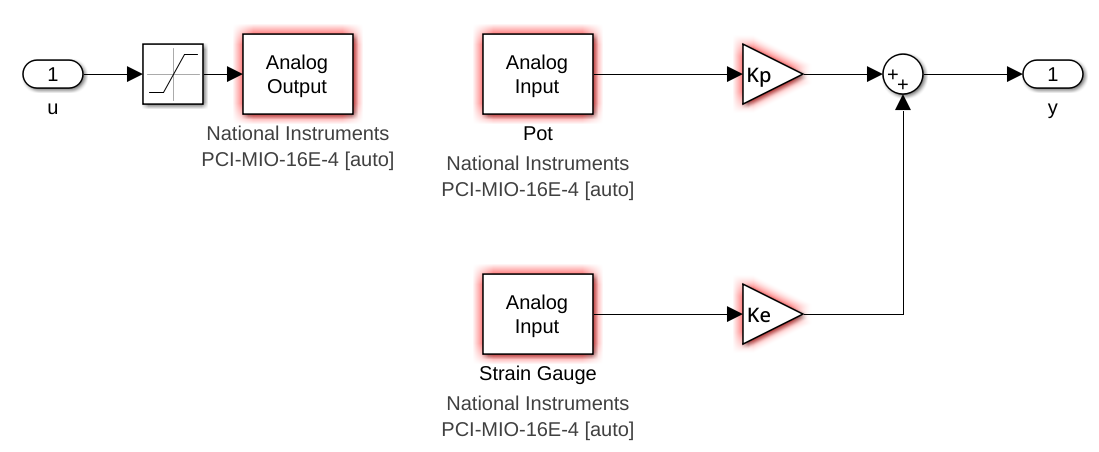
\includegraphics[width=\textwidth]{Figs/Simulink Models/Plant Interface.png}
        \caption{Plant interface}
        \label{fig:plant_interface}
    \end{subfigure}
    \hfill
    \begin{subfigure}{0.37\textwidth}
        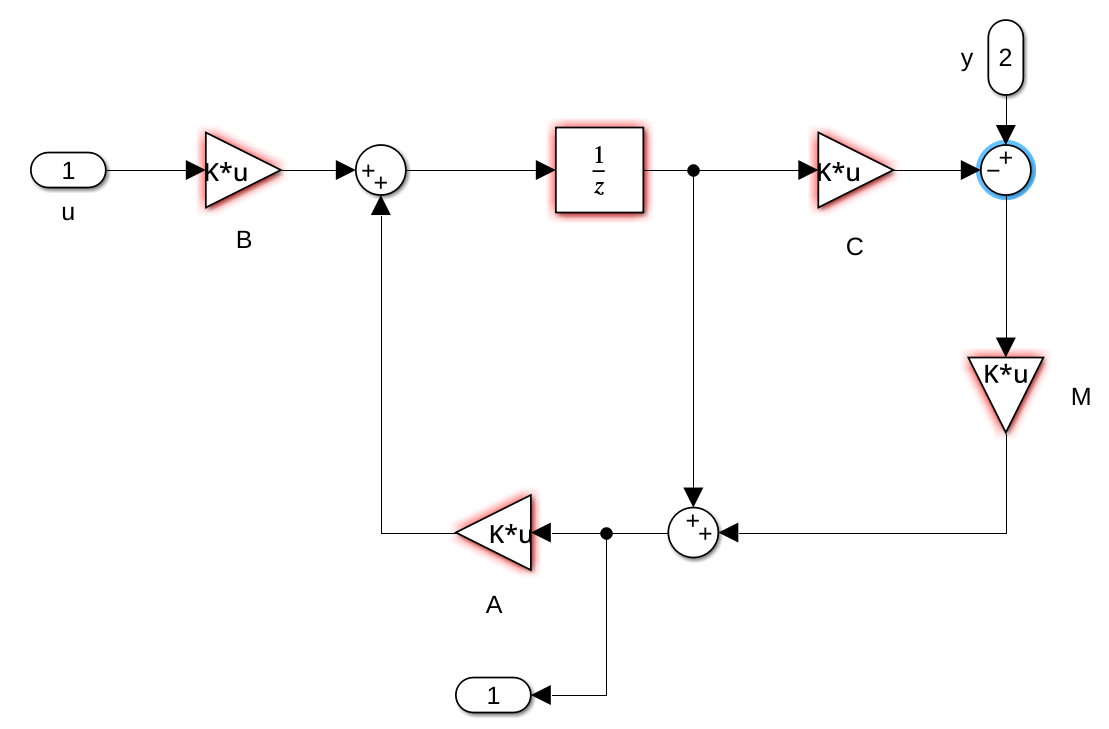
\includegraphics[width=\textwidth]{Figs/Simulink Models/State_Estimator.png}
        \caption{State Estimator}
        \label{fig:state_estimator}
    \end{subfigure}
    \begin{subfigure}{0.95\textwidth}
        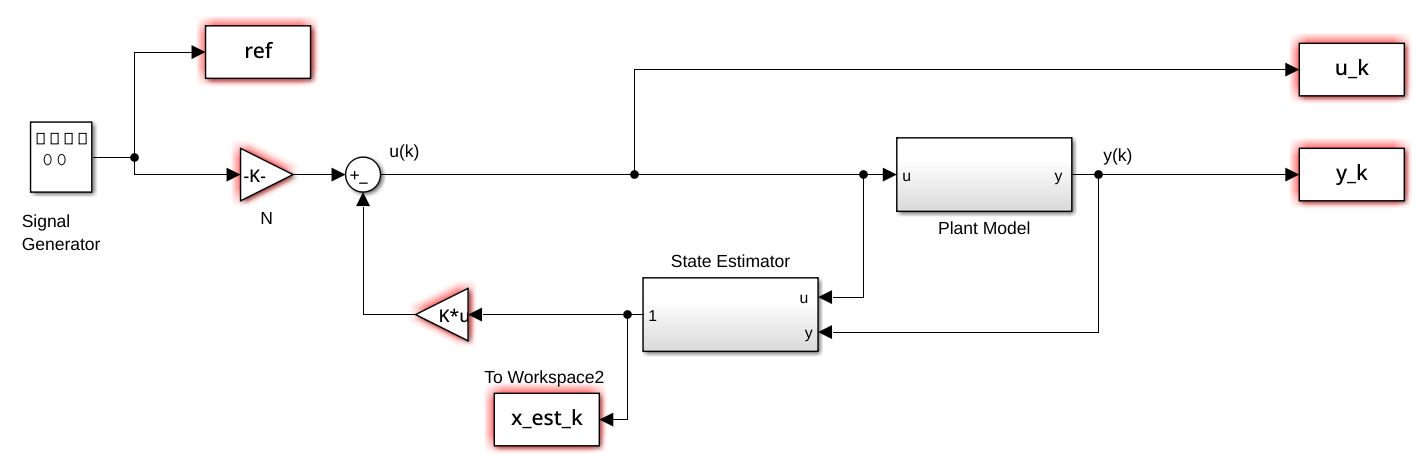
\includegraphics[width=0.9\textwidth]{Figs/Simulink Models/Controller_without_integrator.png}
        \caption{Controller without integrator}
        \label{fig:controller_without_integrator}
    \end{subfigure}
    \caption{Simulink models utilized for system control without integral action}
    \label{fig:simulink_models_no_integrator}
\end{figure}


\begin{figure}[H]
    \centering
    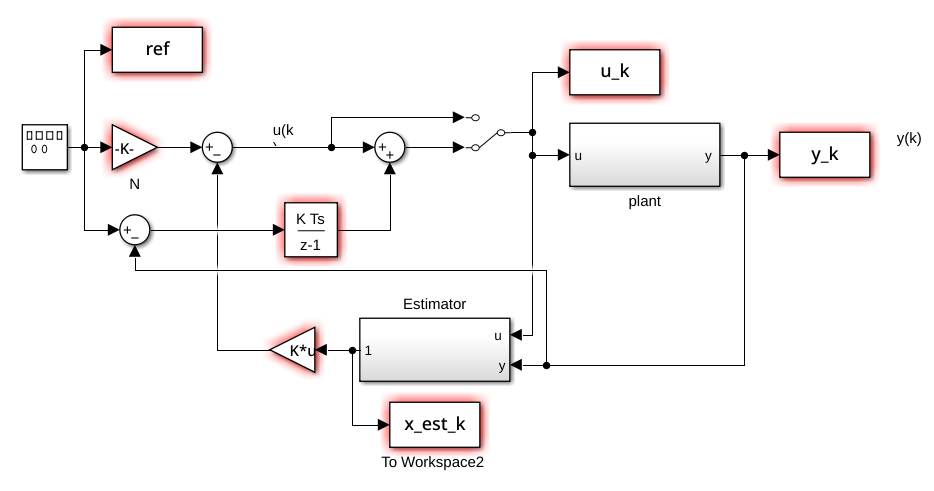
\includegraphics[width=0.7\textwidth]{Figs/Simulink Models/controller_with_integrator.png}
    \caption{Controller with integrator}
    \label{fig:controler_with_integrator}
\end{figure}

%___________________________ Q 4.3 ______________________________
\subsection{Comment on the choice of the weights on the quadratic cost when using the LQG design approach. Include the root-square locus. (3 pts)}
\vspace{10pt}

%%Write your answer here
%___________________________ Q 4.4 ______________________________
\subsection{Explain the effect of the choice of the noise covariance matrices in a LTR framework; (3 pts)}
\vspace{10pt}

%%Write your answer here

In a LTR framework, the choice of noise covariance matrices plays a crucial role in the performance of the system. The process noise covariance matrix $Q$ defines the uncertainty associated to the state dynamics of the system and the choice of a larger $Q$ suggests that the system is being exposed to more significant disturbances in the model. This means that the Kalman filter will value more the measurements performed by the sensors, potentially leading to faster adjustments in the controller. On the other hand, the measurement noise covariance matrix $R$ gives us the uncertainty in the measurements obtained from the sensors and the choice of a larger $R$ suggests more noise in the measurements. This means that, in this case, the Kalman filter will trust more the predictions produced by the model than the measurements.
%___________________________ Q 4.5 ______________________________
\subsection{Display and analyze the resulting closed-loop frequency response and time response. (3 pts)}
\vspace{10pt}

%%Write your answer here
%___________________________ Q 4.6 ______________________________
\subsection{Comment on effect of the inclusion of a pre-filter. (2 pts)}
\vspace{10pt}

%%Write your answer here

Pre-filtering can play a vital role in shaping the reference signal before it enters the feedback loop by adjusting the input signal to compensate any new dynamics introduced by the controller or the plant. 

In this project, different kinds of pre-filters were used to achieve a more accurate positioning of the tip of the robot arm joint. One of them was an integrator, which was used to eliminate the steady-state error and push the system toward the desired output. Another example of the usage of pre-filters in our project are the gain adjustments introduced, which convert the signal's amplitude before entering specific parts of the system. By fine-tuning and using these pre-filters in our system, it is possible to reach the desired positions more quickly and accurately without having a big influence of noise/delays, therefore resulting in better overall performance.
%___________________________ Q 4.7 ______________________________
\subsection{Discuss how do you evaluate the performance of your control system and what are the limits of performance. (3 pts)}
\vspace{10pt}

%%Write your answer here

Our objective for this part of the course was to be able to control the position of the tip of a robotic arm. This came with some chalenges, the first one being that the object used to represent the arm, was a thin metal ruller that was not very rigid, meaning oscilation would happen whenever we moved, the second was the existance of dead zone in the motor and gearbox, this dead zone meant that for small values of the control signal the system would not react, meaning that the system would not reach the desired position, but would stop close to it, and the third main problem we had to deal with was the fact that we were trying to control a linearized version of our system, but the real system was not a linear one, this would induce errors in our model, and would make the system harder to control.

Knowing this we can define two metrics for evaluating the performance of our control system, the first one is how accurate and how fast we can track a desired reference and the second one is how much we can handle big disturbances, such as an object coliding with the arm. Other metrics could be used depending on the application, for example, for a robot where energy is limited, it may be more important to minimize the energy used to reach a position rather than how accurate we track said position.

The limits of performance of our control system are mainly non linear effects that are not taken into consideration in our model, such as the lack of rigidity from the arm, or the dead zone in the motor and gearbox. Also since we are using a discrete time controller, we will also have the problem of only controling  the system in certain time steps, meaning that is for some reason we acheive an oscilation of aroungd 50Hz, our sampling rate, we would not be able to detecte it, meaning we would not stop it. Also, there is a limit for the speed of the system, since the both the motor and the arm have a maximum speed, the motor due to the voltage safety limits, and the arm due to the lack of rigidity and the air resistance.

After considering how we could evaluate our system and its performance limits, we now present the plots from Figure \ref{fig: Performance Plots}. 
On the left, Figure \ref{fig: Reference Tracking}, the system response accurately tracks the reference, requiring approximately 4 seconds to follow a 90-degree change in reference. 
Notably, the first 96\% of the change is achieved within the first 0.5 seconds, which is an excellent result. The system stops initially at 41.6 degrees, very close to the target of 45 degrees.

On the right, Figure \ref{fig: Disturbance Handling}, we observe the system's response to multiple disturbances (three in total). The first disturbance occurs slightly after the 5-second mark, and the system returns within 5 degrees of the target in under a second after releasing the arm. 
However, the reference error is not fully eliminated as a new disturbance occurs at the 9-second mark. In both this disturbance and the next, at 15 seconds, the system again reduces the deviation to within 5 degrees of the target in about 0.5 seconds. 
Furthermore, as observed earlier, it takes approximately 3.5 seconds after reaching this plateau for the system to achieve the reference target position.


\begin{figure}
    \centering
    \begin{subfigure}{0.45\textwidth}
        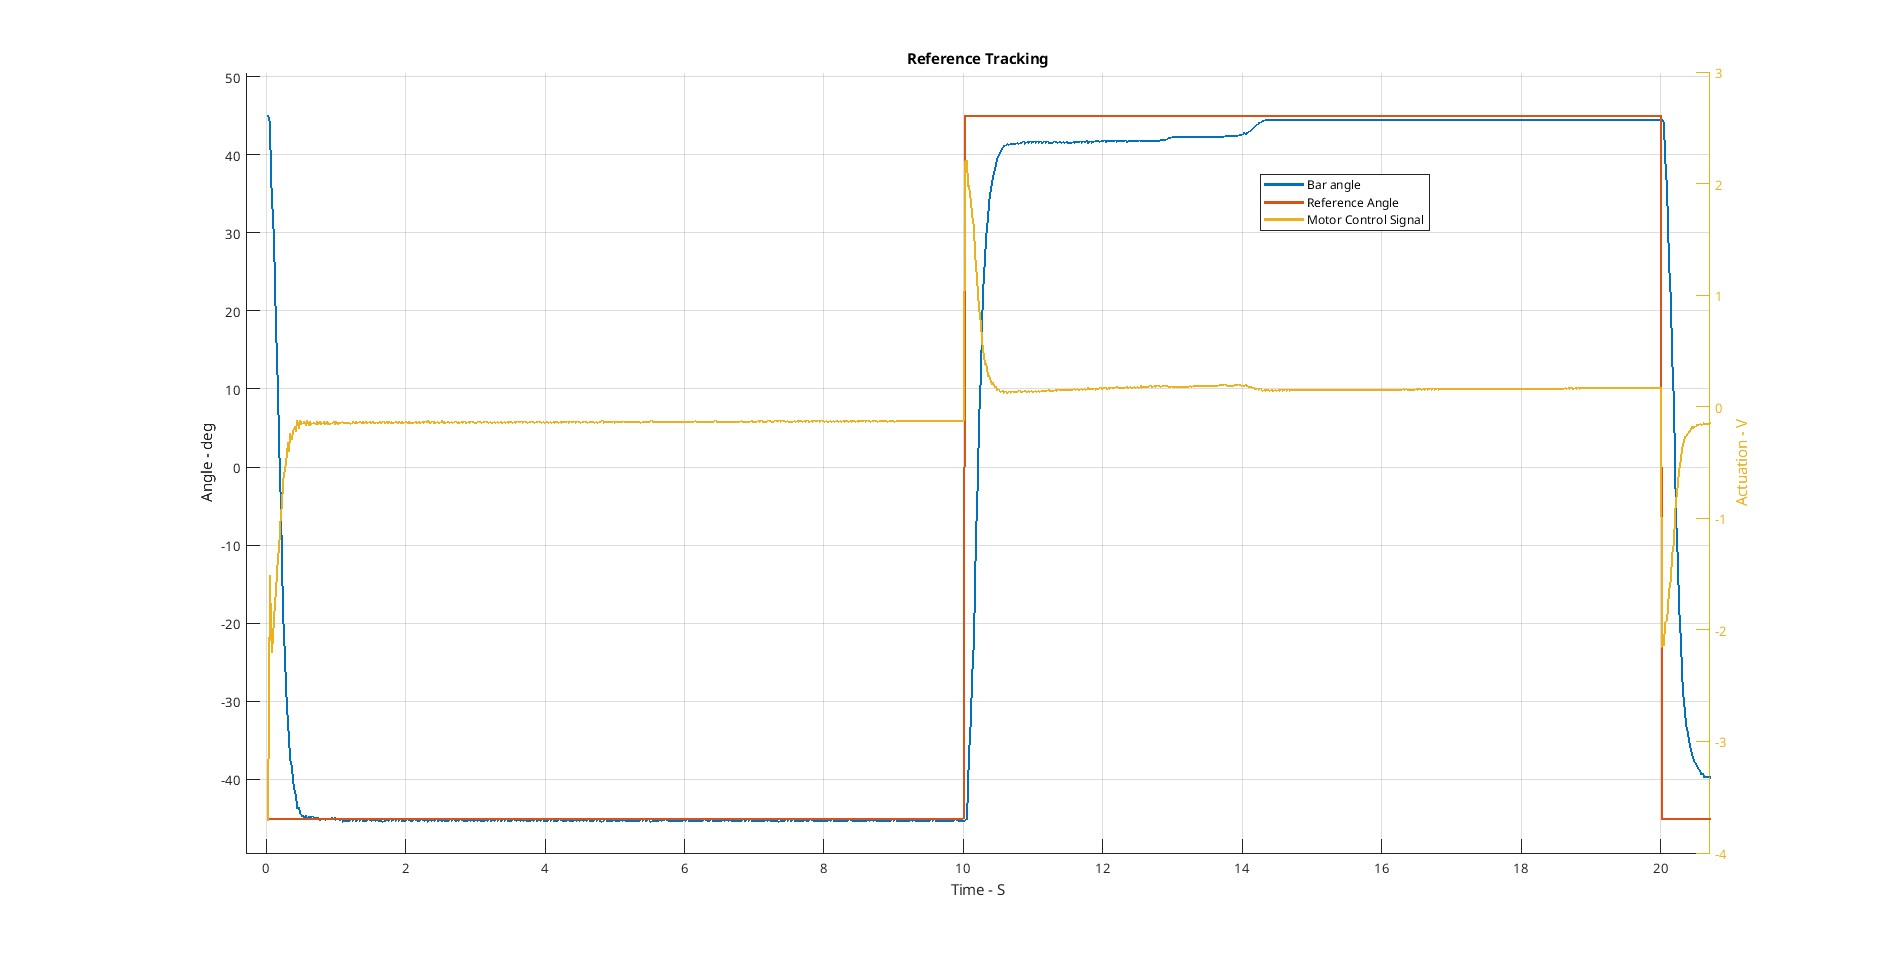
\includegraphics[width=\textwidth]{Figs/Reference Tracking.jpg} 
        \caption{Reference Tracking}
        \label{fig: Reference Tracking} 
    \end{subfigure}
    \hfill
    \begin{subfigure}{0.45\textwidth}
        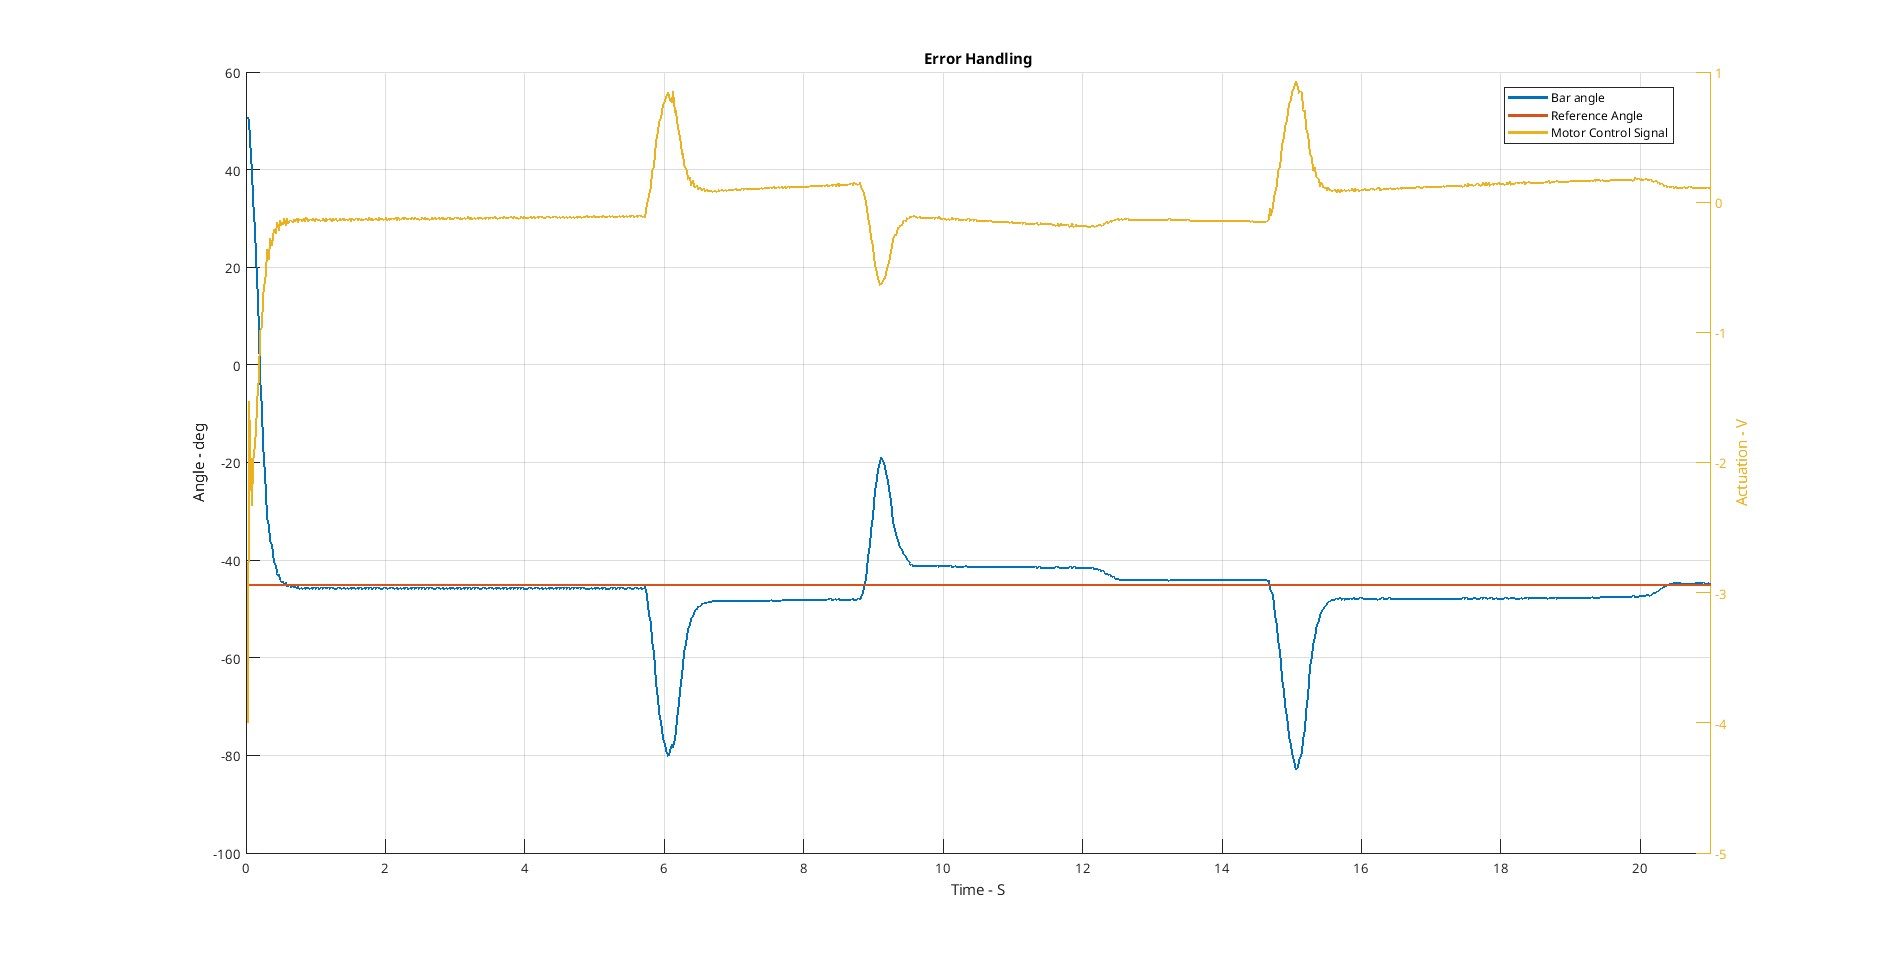
\includegraphics[width=\textwidth]{Figs/Error handling.jpg} 
        \caption{Disturbance handling}
        \label{fig: Disturbance Handling}
    \end{subfigure}
    \caption{Plots showing the performance of the control system}
    \label{fig: Performance Plots}
\end{figure}

\addcontentsline{toc}{section}{{Conclusions}}
\section*{Conclusions}

This project successfully achieved the design and implementation of a control system for a flexible robot arm joint. By applying Linear Quadratic Gaussian (LQG) control and Kalman filtering, the system was able to precisely control the positioning of the flexible bar, while maintaining stability and addressing uncertainties.

Through testing and validation, the controller demonstrated effective performance, meeting the required criteria in both time and frequency domains. The use of Loop Transfer Recovery (LTR) further improved the system’s robustness, ensuring that it could handle disturbances.

Overall, this work illustrates the practical use of advanced control techniques in managing cyber-physical systems. The documentation, along with the MATLAB scripts and Simulink models, offers a solid basis for future enhancements and further development.


\end{document}